\chapter{Model Scaling and Efficiency}

Every architectural finding in Chapters~4--6 was established at a single, fixed model size. This chapter examines how classifier performance and inference cost vary across a factor of roughly 140 in parameter count, from approximately 26k to 3.6M parameters. Two questions motivate this study. First, where does AUROC saturate as a function of model capacity, and does the saturation point shift with task difficulty? Second, which configuration is Pareto-optimal when performance is weighed against inference cost? The answers retrospectively validate the fixed size used throughout Chapters~4--6 and identify a practical operating point for the evaluation in Chapter~8.

The chapter is structured as follows. Section~\ref{sec:ch7_design} describes the experimental design, which is a full factorial sweep of five model-size presets across three classification tasks (Exp.~7A). Section~\ref{sec:ch7_scaling} reports performance as a function of model size and training cost. Section~\ref{sec:ch7_pareto} presents the Pareto analysis across four efficiency dimensions (Exp.~7B). Section~\ref{sec:ch7_summary} summarises the findings.

% ──────────────────────────────────────────────
\section{Experimental Design}
\label{sec:ch7_design}

All 45 runs in this chapter share a common fixed baseline configuration: tokenizer family \texttt{identity} (axis T1), the feature set D01 selected in Chapter~4, sinusoidal positional encoding (E1 = \texttt{sinusoidal}), standard attention (A3 = \texttt{standard}), LayerNorm with pre-norm policy (A1, A2), and no physics-informed attention biases (B1 = \texttt{none}). Model capacity is the sole variable, swept via the convenience label axis \wandbaxis{H10}, which bundles model dimension (\wandbaxis{H01}), encoder depth (\wandbaxis{H02}), attention heads (H03), and FFN hidden dimension (H04) into five named presets. Three random seeds per cell (axis R05) give 45 runs in total.

\begin{table}[h]
\centering\small
\caption{Exp.~7A design. All other axes held at their thesis baseline values.}
\label{tab:ch7_design}
\begin{tabular}{lll}
\toprule
Axis & Values & Cells \\
\midrule
Model size (\wandbaxis{H10}) & \texttt{d32\_L3}, \texttt{d32\_L5}, \texttt{d64\_L6},
                              \texttt{d128\_L8}, \texttt{d192\_L12} & 5 \\
Task (G03)       & 4t\,vs.\,background, 4t\,vs.\,ttH, multiclass & 3 \\
Seed (R05)       & 3 per cell & 3 \\
\midrule
Total & & \textbf{45} \\
\bottomrule
\end{tabular}
\end{table}

Table~\ref{tab:ch7_sizes} lists the concrete dimension and depth values for each preset, together with the approximate parameter count and analytic FLOPs per event. Analytic FLOPs count multiply-add operations derived from the model architecture; they do not include Python overhead or data-movement costs, but provide a clean, hardware-independent comparison basis.

\begin{table}[h]
\centering\small
\caption{Model-size presets used in Exp.~7A. Approximate parameter counts are derived from H01 and H02; FLOPs per event are analytic multiply-add counts averaged over all 9 runs sharing that preset.}
\label{tab:ch7_sizes}
\begin{tabular}{lrrrl}
\toprule
Size label (H10) & dim (H01) & depth (H02) & Approx.\ params & FLOPs/event (analytic) \\
\midrule
\texttt{d32\_L3}   & 32  & 3  & $\sim$26k   & 1.29M \\
\texttt{d32\_L5}   & 32  & 5  & $\sim$43k   & 2.15M \\
\texttt{d64\_L6}   & 64  & 6  & $\sim$202k  & 10.3M \\
\texttt{d128\_L8}  & 128 & 8  & $\sim$1.06M & 55.1M \\
\texttt{d192\_L12} & 192 & 12 & $\sim$3.57M & 185.8M \\
\bottomrule
\end{tabular}
\end{table}

The jump in FLOPs from \texttt{d64\_L6} to \texttt{d128\_L8} is approximately $\times 5.3$, and from \texttt{d64\_L6} to \texttt{d192\_L12} approximately $\times 18$. This non-linear growth is driven by the quadratic attention cost and the multiplicative effect of simultaneously increasing both depth and width.

% ──────────────────────────────────────────────
\section{Scaling Curves (Exp.\ 7A)}
\label{sec:ch7_scaling}

\subsection{AUROC versus Model Size}

Figure~\ref{fig:ch7_auroc} shows AUROC as a function of model size, separately for each task and aggregated over all three tasks. The aggregated mean and standard deviation over all nine runs (three tasks $\times$ three seeds) per size are reported in Table~\ref{tab:ch7_auroc}.

\begin{figure}[h]
  \centering
  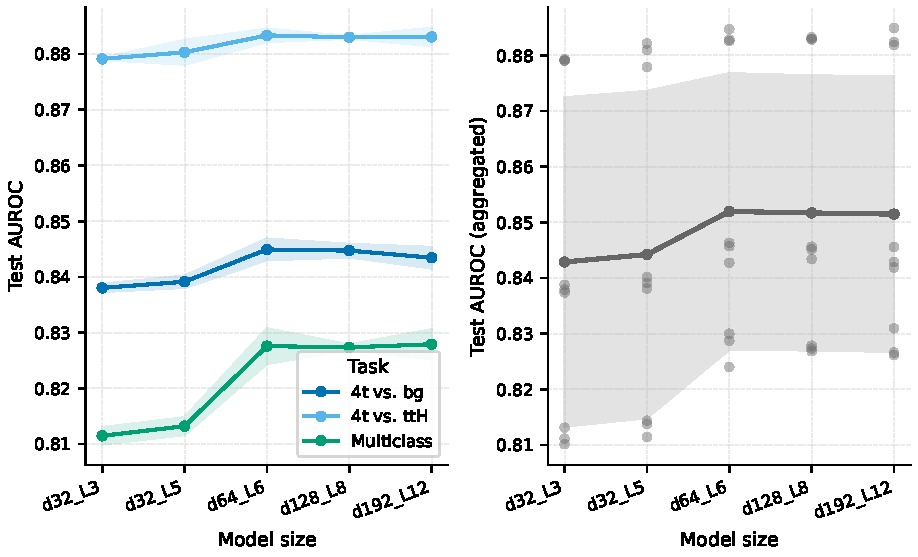
\includegraphics[width=\linewidth]{figures/ch7/ch7_auroc_vs_model_size.pdf}
  \caption{AUROC versus model-size preset for all three tasks (left) and aggregated over tasks with seed scatter (right); higher AUROC is better, and the plateau at \texttt{d64\_L6} is visible in both panels.}
  \label{fig:ch7_auroc}
\end{figure}

\begin{table}[h]
\centering\small
\caption{Aggregated AUROC by model-size preset (mean $\pm$ std over all 9 runs, 3 tasks $\times$ 3 seeds). The large standard deviation reflects cross-task variance, not seed noise; within a single task, seed-to-seed variation is substantially smaller.}
\label{tab:ch7_auroc}
\begin{tabular}{lrr}
\toprule
Size label (H10) & Mean AUROC & Std \\
\midrule
\texttt{d32\_L3}   & 0.843 & 0.030 \\
\texttt{d32\_L5}   & 0.844 & 0.029 \\
\texttt{d64\_L6}   & 0.852 & 0.025 \\
\texttt{d128\_L8}  & 0.852 & 0.025 \\
\texttt{d192\_L12} & 0.852 & 0.025 \\
\bottomrule
\end{tabular}
\end{table}

AUROC rises by approximately 0.8--1.3 percentage points between the two smallest presets and \texttt{d64\_L6}, but the three larger configurations (\texttt{d64\_L6}, \texttt{d128\_L8}, \texttt{d192\_L12}) are statistically indistinguishable at $0.852 \pm 0.025$. The plateau is consistent across all three tasks in the per-task panel. Although the multiclass task yields systematically lower absolute AUROC than the binary tasks (owing to the harder five-class discriminant), the saturation point does not shift: all three tasks plateau at \texttt{d64\_L6}.

The saturation at this relatively small scale is consistent with the low-multiplicity nature of the classification problem. Events in the 4t and ttH samples contain at most a few tens of reconstructed objects, so the information content available per event is modest, and a model with $\sim$202k parameters appears sufficient to extract it with the baseline architecture.

\paragraph{Signal efficiency at fixed background rejection.}

For the two binary tasks, signal efficiency $\varepsilon_S$ at a fixed background rejection of $1/B = 50$ provides a physics-operational complement to AUROC. This metric is undefined for the multiclass task and is not reported there. Table~\ref{tab:ch7_eps} summarises the results.

\begin{table}[h]
\centering\small
\caption{Signal efficiency $\varepsilon_S$ at background rejection $1/B = 50$, for the two binary tasks (mean $\pm$ std over 3 seeds). The plateau pattern mirrors the AUROC result.}
\label{tab:ch7_eps}
\begin{tabular}{lrr}
\toprule
Size label (H10) & $\varepsilon_S$, 4t vs.\ bg & $\varepsilon_S$, 4t vs.\ ttH \\
\midrule
\texttt{d32\_L3}   & $0.276 \pm 0.006$ & $0.283 \pm 0.003$ \\
\texttt{d32\_L5}   & $0.277 \pm 0.000$ & $0.284 \pm 0.005$ \\
\texttt{d64\_L6}   & $0.284 \pm 0.002$ & $0.298 \pm 0.008$ \\
\texttt{d128\_L8}  & $0.286 \pm 0.009$ & $0.290 \pm 0.007$ \\
\texttt{d192\_L12} & $0.288 \pm 0.004$ & $0.292 \pm 0.007$ \\
\bottomrule
\end{tabular}
\end{table}

At \texttt{d64\_L6}, $\varepsilon_S \approx 0.284$ for 4t\,vs.\,background and $\varepsilon_S \approx 0.298$ for 4t\,vs.\,ttH. The larger models do not improve on these values by a statistically meaningful margin. The values at $1/B = 1000$ were inspected but are non-monotone across model sizes, reflecting the sparsity of events at very high rejection; this threshold is not informative for architectural comparisons and is not used as a primary metric in this chapter.

\subsection{Training Cost}

Figure~\ref{fig:ch7_wallclock} shows total training wall-clock time as a function of model-size preset, and Figure~\ref{fig:ch7_epoch} shows the best checkpoint epoch at which early stopping triggered. Figure~\ref{fig:ch7_flops} shows the analytic FLOPs per event on a log-log scale against parameter count.

\begin{figure}[h]
  \centering
  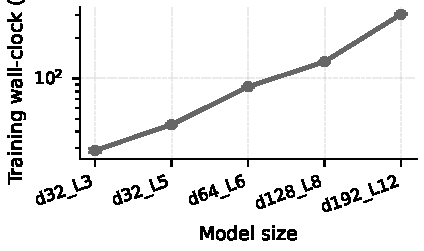
\includegraphics[width=\linewidth]{figures/ch7/ch7_wallclock_vs_model_size.pdf}
  \caption{Total training wall-clock time (seconds) versus model-size preset on a logarithmic vertical axis; lower is faster, and the approximately linear growth with parameter count is consistent with FLOPs scaling.}
  \label{fig:ch7_wallclock}
\end{figure}

\begin{figure}[h]
  \centering
  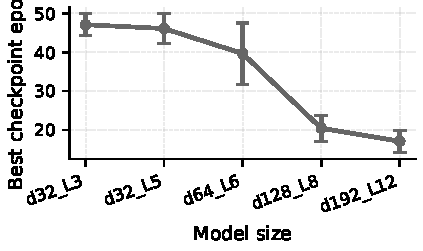
\includegraphics[width=\linewidth]{figures/ch7/ch7_epoch_vs_model_size.pdf}
  \caption{Best checkpoint epoch (early-stopping trigger) versus model-size preset; larger models converge in fewer epochs, but each epoch takes longer, so total wall-clock time still grows with model size.}
  \label{fig:ch7_epoch}
\end{figure}

\begin{figure}[h]
  \centering
  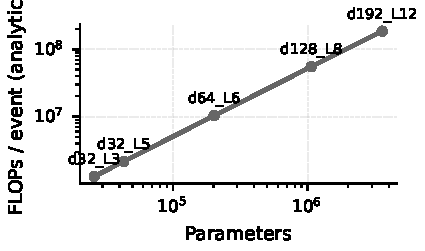
\includegraphics[width=\linewidth]{figures/ch7/ch7_flops_vs_model_size.pdf}
  \caption{Analytic FLOPs per event versus approximate parameter count on a log-log scale; the non-linear growth reflects the simultaneous increase in model dimension and depth across presets.}
  \label{fig:ch7_flops}
\end{figure}

Table~\ref{tab:ch7_training} summarises the training cost metrics. Wall-clock time grows from 28.9\,s at \texttt{d32\_L3} to 302.7\,s at \texttt{d192\_L12}, a factor of approximately $10.5\times$. Over the same range, analytic FLOPs per event grow by a factor of approximately $144\times$ (from 1.29M to 185.8M). The discrepancy between the FLOPs ratio and the wall-clock ratio reflects the fact that wall-clock time includes evaluation and benchmarking overhead (latency measurement), which is size-independent and inflates the cost of smaller models. The best-epoch trend shows an inverse relationship with model size: larger models trigger early stopping sooner (mean epoch 17 for \texttt{d192\_L12} versus 47 for \texttt{d32\_L3}), because their greater capacity results in faster loss descent per epoch. However, each epoch is considerably more expensive for the larger models, so the total wall-clock time is dominated by per-epoch cost for \texttt{d192\_L12}.

\begin{table}[h]
\centering\small
\caption{Training cost metrics by model-size preset (mean $\pm$ std over 9 runs, 3 tasks $\times$ 3 seeds). Wall-clock includes evaluation overhead; best epoch is the early-stopping trigger.}
\label{tab:ch7_training}
\begin{tabular}{lrrr}
\toprule
Size label (H10) & Wall-clock (s) & Best epoch & FLOPs/event (analytic) \\
\midrule
\texttt{d32\_L3}   & $28.9 \pm 0.8$  & $47.1 \pm 2.8$ & 1.29M \\
\texttt{d32\_L5}   & $45.1 \pm 0.8$  & $46.1 \pm 3.8$ & 2.15M \\
\texttt{d64\_L6}   & $86.7 \pm 0.7$  & $39.7 \pm 7.9$ & 10.3M \\
\texttt{d128\_L8}  & $133.5 \pm 1.0$ & $20.4 \pm 3.4$ & 55.1M \\
\texttt{d192\_L12} & $302.7 \pm 1.6$ & $17.1 \pm 2.8$ & 185.8M \\
\bottomrule
\end{tabular}
\end{table}

% ──────────────────────────────────────────────
\section{Efficiency and Pareto Analysis (Exp.\ 7B)}
\label{sec:ch7_pareto}

Experiment~7B repurposes the 45 checkpoints from Exp.~7A to measure four inference-side efficiency metrics at batch size 512: latency per batch, throughput in samples per second, and peak memory allocation. These are plotted in Pareto space against AUROC in Figures~\ref{fig:ch7_pareto_flops}--\ref{fig:ch7_pareto_memory}. In each panel, a point on the Pareto frontier represents a configuration for which no other configuration achieves higher AUROC at lower cost. No new training was required for Exp.~7B; all metrics were recorded during the evaluation phase of Exp.~7A and are available in the canonical run table with zero missing values.

Batch size 512 is the primary efficiency reference because single-event latency (batch size 1) exhibits large standard deviations for \texttt{d64\_L6} and \texttt{d128\_L8} ($\sigma \approx 1.2$--1.6\,ms), attributable to operating-system scheduling jitter on the interactive node rather than model variability. At batch size 512, standard deviations are below 0.02\,ms across all presets, making the measurements far more reproducible.

\paragraph{AUROC versus FLOPs per event.}

Figure~\ref{fig:ch7_pareto_flops} shows AUROC against analytic FLOPs per event per task and aggregated. The gap between the two smallest presets and \texttt{d64\_L6} is visible in AUROC but represents only a factor of approximately 8 in FLOPs ($1.29$M to $10.3$M). Above \texttt{d64\_L6}, AUROC is flat while FLOPs increase by a factor of $\times 18$ to reach \texttt{d192\_L12} at 185.8M FLOPs per event. \texttt{d64\_L6} lies on the Pareto frontier: no larger model improves AUROC, and no smaller model matches its AUROC at lower cost.

\begin{figure}[h]
  \centering
  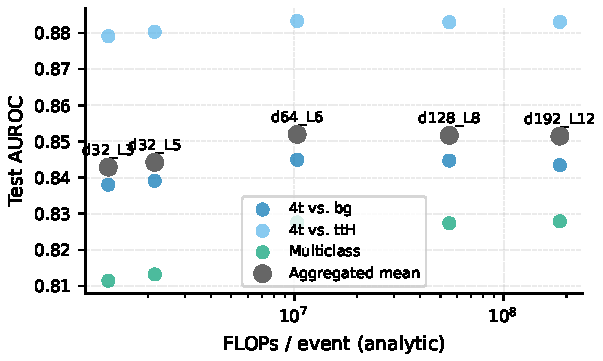
\includegraphics[width=\linewidth]{figures/ch7/ch7_pareto_auroc_vs_flops.pdf}
  \caption{AUROC versus analytic FLOPs per event per task (left) and aggregated (right); points further up and to the left are Pareto-preferable, and \texttt{d64\_L6} lies on the frontier.}
  \label{fig:ch7_pareto_flops}
\end{figure}

\paragraph{AUROC versus inference latency.}

Figure~\ref{fig:ch7_pareto_latency} shows AUROC against per-batch inference latency at batch size 512. Table~\ref{tab:ch7_inference} reports the numeric values. Latency grows from 0.163\,ms at \texttt{d32\_L3} to 2.019\,ms at \texttt{d192\_L12}, a factor of approximately $12.4\times$. The latency of \texttt{d64\_L6} (0.552\,ms) is $3.7\times$ lower than that of \texttt{d192\_L12} at identical AUROC. Again, \texttt{d64\_L6} sits on the Pareto frontier.

\begin{figure}[h]
  \centering
  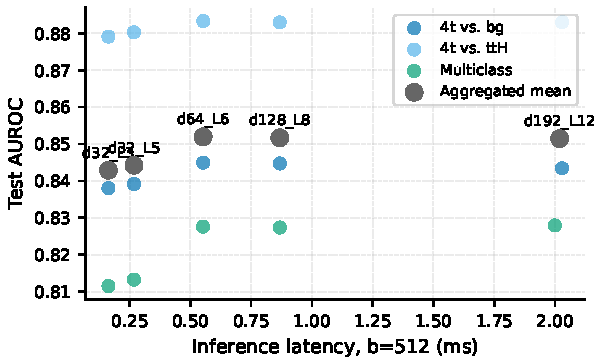
\includegraphics[width=\linewidth]{figures/ch7/ch7_pareto_auroc_vs_latency.pdf}
  \caption{AUROC versus inference latency per batch at batch size 512 (ms); lower latency and higher AUROC are jointly preferable, with \texttt{d64\_L6} on the frontier.}
  \label{fig:ch7_pareto_latency}
\end{figure}

\paragraph{AUROC versus throughput.}

Figure~\ref{fig:ch7_pareto_throughput} shows AUROC against throughput in samples per second. Throughput drops from approximately 3.14M samples/s at \texttt{d32\_L3} to 927k samples/s at \texttt{d64\_L6} and 254k samples/s at \texttt{d192\_L12}. Because the larger models provide no AUROC improvement over \texttt{d64\_L6}, the throughput reduction by a further factor of $3.7\times$ from \texttt{d64\_L6} to \texttt{d192\_L12} is not compensated by any discriminative gain. Although \texttt{d32\_L3} and \texttt{d32\_L5} offer higher throughput than \texttt{d64\_L6}, they sacrifice approximately 1 percentage point of AUROC, which corresponds to a measurable reduction in $\varepsilon_S$ at operational background rejection rates.

\begin{figure}[h]
  \centering
  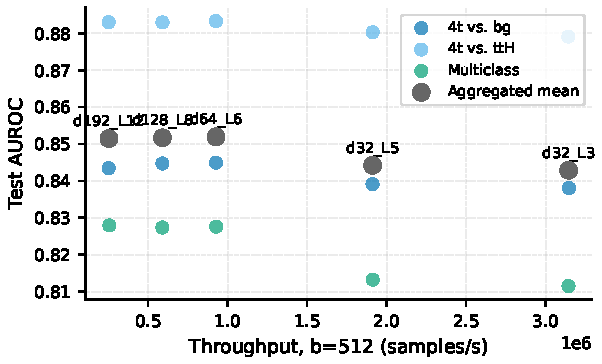
\includegraphics[width=\linewidth]{figures/ch7/ch7_pareto_auroc_vs_throughput.pdf}
  \caption{AUROC versus inference throughput at batch size 512 (samples/s); higher throughput and higher AUROC are jointly preferable, with \texttt{d64\_L6} on the frontier.}
  \label{fig:ch7_pareto_throughput}
\end{figure}

\paragraph{AUROC versus peak memory.}

Figure~\ref{fig:ch7_pareto_memory} shows AUROC against peak inference memory at batch size 512. Memory grows from approximately 996\,MiB at \texttt{d32\_L3} and \texttt{d32\_L5} (nearly identical, as the MiB allocation is dominated by batch and activation buffers) to 1,968\,MiB at \texttt{d64\_L6}, 3,187\,MiB at \texttt{d128\_L8}, and 4,772\,MiB at \texttt{d192\_L12}. Memory standard deviations are negligible across all presets, reflecting deterministic allocation independent of random seed. The $\times 2.4$ memory increase from \texttt{d64\_L6} to \texttt{d192\_L12} accompanies no improvement in AUROC, confirming \texttt{d64\_L6} as Pareto-optimal on this dimension as well.

\begin{figure}[h]
  \centering
  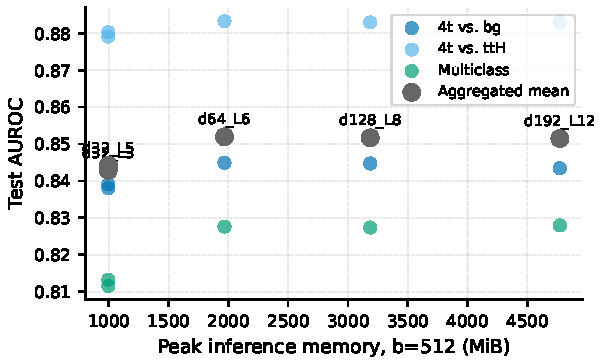
\includegraphics[width=\linewidth]{figures/ch7/ch7_pareto_auroc_vs_memory.pdf}
  \caption{AUROC versus peak inference memory at batch size 512 (MiB); lower memory and higher AUROC are jointly preferable, and \texttt{d64\_L6} lies on the frontier in all task panels.}
  \label{fig:ch7_pareto_memory}
\end{figure}

\begin{table}[h]
\centering\small
\caption{Inference efficiency metrics at batch size 512 by model-size preset (mean $\pm$ std over 9 runs). Memory standard deviations are $<$0.1\,MiB and are omitted.}
\label{tab:ch7_inference}
\begin{tabular}{lrrr}
\toprule
Size label (H10) & Latency (ms) & Throughput (samples/s) & Peak memory (MiB) \\
\midrule
\texttt{d32\_L3}   & $0.163 \pm 0.000$ & 3,145k & 996  \\
\texttt{d32\_L5}   & $0.268 \pm 0.000$ & 1,912k & 996  \\
\texttt{d64\_L6}   & $0.552 \pm 0.001$ &   927k & 1,968 \\
\texttt{d128\_L8}  & $0.868 \pm 0.001$ &   590k & 3,187 \\
\texttt{d192\_L12} & $2.019 \pm 0.015$ &   254k & 4,772 \\
\bottomrule
\end{tabular}
\end{table}

Across all four Pareto dimensions — FLOPs per event, inference latency, throughput, and peak memory — \texttt{d64\_L6} ($\sim$202k parameters, $\sim$10.3M FLOPs per event) is the Pareto-optimal configuration for this task family. It achieves the full discriminative performance of models up to $\times 18$ more expensive in FLOPs and $\times 3.7$ slower in latency.

% ──────────────────────────────────────────────
\section*{Chapter Summary}
\label{sec:ch7_summary}

\begin{table}[h]
\centering\small
\caption{Chapter~7 experiment summary.}
\label{tab:ch7_summary}
\begin{tabular}{llr}
\toprule
Experiment & Description & Runs \\
\midrule
7A — Scaling curves  & 5 sizes $\times$ 3 tasks $\times$ 3 seeds & 45 \\
7B — Pareto analysis & Post-hoc efficiency metrics from Exp.~7A checkpoints & 0 \\
\midrule
\textbf{Total} & & \textbf{45} \\
\bottomrule
\end{tabular}
\end{table}

AUROC saturates at \texttt{d64\_L6} ($\sim$202k parameters) and does not improve for the three larger presets, regardless of task. Signal efficiency at fixed background rejection ($1/B = 50$) confirms the same plateau: $\varepsilon_S \approx 0.284$ for 4t\,vs.\,background and $\varepsilon_S \approx 0.298$ for 4t\,vs.\,ttH at \texttt{d64\_L6}, with no statistically significant gain from \texttt{d128\_L8} or \texttt{d192\_L12}. On the inference side, \texttt{d64\_L6} is Pareto-optimal across FLOPs per event, latency, throughput, and peak memory, at batch size 512. This finding retrospectively validates the fixed model size applied throughout Chapters~4--6, and establishes the \texttt{d64\_L6} configuration as the comparison baseline for Chapter~8, which asks which combination of architectural choices drawn from those chapters achieves the highest discrimination performance.

One limitation of this analysis is that the scaling results apply to the baseline architecture only. Whether a better-performing architecture identified in Chapter~8 scales differently — for example, saturating later or earlier — is an open question that falls outside the scope of this thesis.
